برای تابع داده شده، داده‌شده:

\begin{latin}
	$f(a,b,c,d)=\sum m(1,3,4,5,10,11,14,15)$
\end{latin}


\begin{enumerate}
	\item
	ابتدا آن را به ساده‌ترین فرم \lr{SOP} بنویسید، سپس موج خروجی را به ازای گذار «صفحه بعد» رسم کنید. (تاخیر گیت های یک ورودی، دو ورودی و سه ورودی به‌ترتیب 3 و 4 و 5 نانوثانیه می‌باشد)
	
	
	\begin{figure}[h]
		\centering
		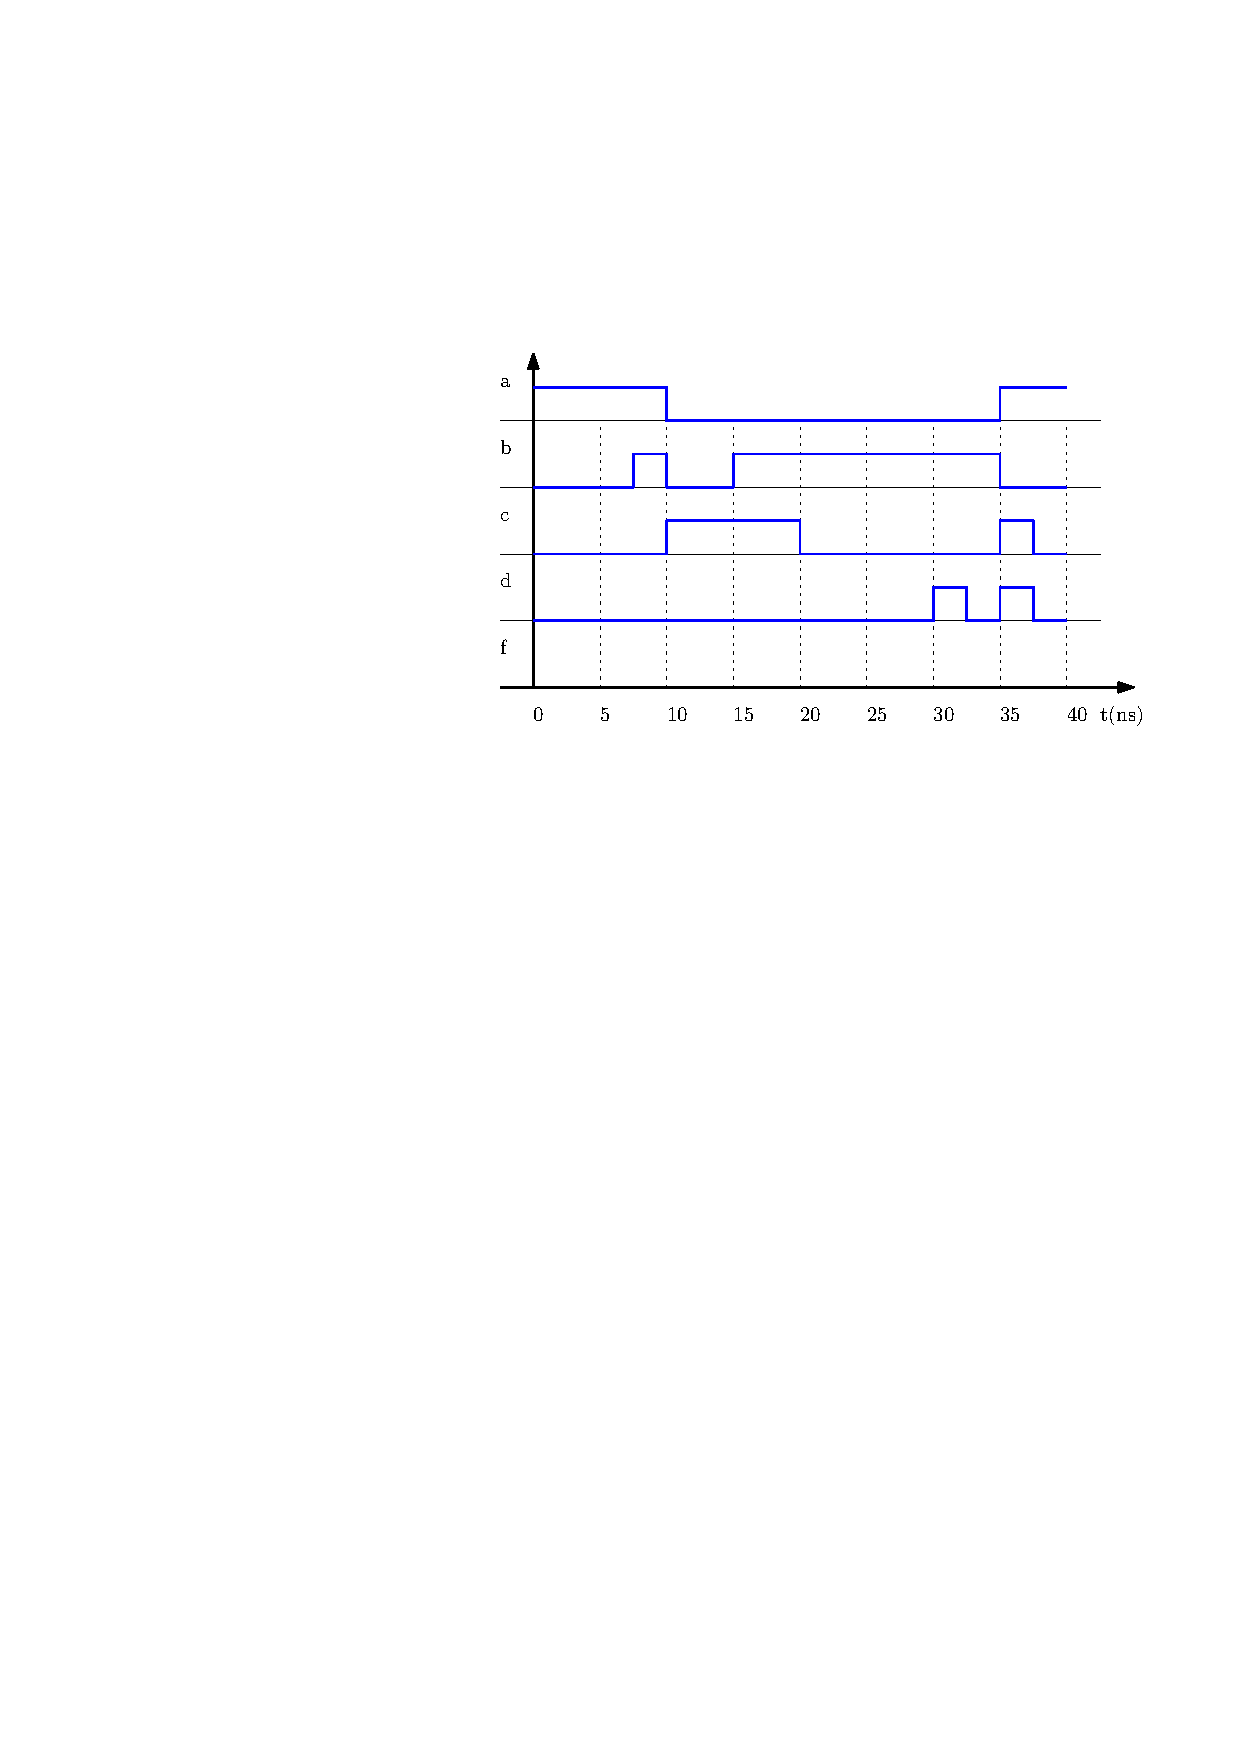
\includegraphics[width=1\textwidth]{fig/Q8.pdf}
		\label{fig:Q8}
		\caption{گذار سوال ۸}
	\end{figure}
	
	
	
	
	\item 
	با ذکر دلیل تعیین کنید که آیا مدار گلیچ می گیرد یا خیر. 
\end{enumerate}